\documentclass[]{article}
\usepackage{lmodern}
\usepackage{amssymb,amsmath}
\usepackage{ifxetex,ifluatex}
\usepackage{fixltx2e} % provides \textsubscript
\ifnum 0\ifxetex 1\fi\ifluatex 1\fi=0 % if pdftex
  \usepackage[T1]{fontenc}
  \usepackage[utf8]{inputenc}
\else % if luatex or xelatex
  \ifxetex
    \usepackage{mathspec}
  \else
    \usepackage{fontspec}
  \fi
  \defaultfontfeatures{Ligatures=TeX,Scale=MatchLowercase}
\fi
% use upquote if available, for straight quotes in verbatim environments
\IfFileExists{upquote.sty}{\usepackage{upquote}}{}
% use microtype if available
\IfFileExists{microtype.sty}{%
\usepackage{microtype}
\UseMicrotypeSet[protrusion]{basicmath} % disable protrusion for tt fonts
}{}
\usepackage[margin=1in]{geometry}
\usepackage{hyperref}
\hypersetup{unicode=true,
            pdftitle={Chap 4},
            pdfborder={0 0 0},
            breaklinks=true}
\urlstyle{same}  % don't use monospace font for urls
\usepackage{color}
\usepackage{fancyvrb}
\newcommand{\VerbBar}{|}
\newcommand{\VERB}{\Verb[commandchars=\\\{\}]}
\DefineVerbatimEnvironment{Highlighting}{Verbatim}{commandchars=\\\{\}}
% Add ',fontsize=\small' for more characters per line
\usepackage{framed}
\definecolor{shadecolor}{RGB}{248,248,248}
\newenvironment{Shaded}{\begin{snugshade}}{\end{snugshade}}
\newcommand{\AlertTok}[1]{\textcolor[rgb]{0.94,0.16,0.16}{#1}}
\newcommand{\AnnotationTok}[1]{\textcolor[rgb]{0.56,0.35,0.01}{\textbf{\textit{#1}}}}
\newcommand{\AttributeTok}[1]{\textcolor[rgb]{0.77,0.63,0.00}{#1}}
\newcommand{\BaseNTok}[1]{\textcolor[rgb]{0.00,0.00,0.81}{#1}}
\newcommand{\BuiltInTok}[1]{#1}
\newcommand{\CharTok}[1]{\textcolor[rgb]{0.31,0.60,0.02}{#1}}
\newcommand{\CommentTok}[1]{\textcolor[rgb]{0.56,0.35,0.01}{\textit{#1}}}
\newcommand{\CommentVarTok}[1]{\textcolor[rgb]{0.56,0.35,0.01}{\textbf{\textit{#1}}}}
\newcommand{\ConstantTok}[1]{\textcolor[rgb]{0.00,0.00,0.00}{#1}}
\newcommand{\ControlFlowTok}[1]{\textcolor[rgb]{0.13,0.29,0.53}{\textbf{#1}}}
\newcommand{\DataTypeTok}[1]{\textcolor[rgb]{0.13,0.29,0.53}{#1}}
\newcommand{\DecValTok}[1]{\textcolor[rgb]{0.00,0.00,0.81}{#1}}
\newcommand{\DocumentationTok}[1]{\textcolor[rgb]{0.56,0.35,0.01}{\textbf{\textit{#1}}}}
\newcommand{\ErrorTok}[1]{\textcolor[rgb]{0.64,0.00,0.00}{\textbf{#1}}}
\newcommand{\ExtensionTok}[1]{#1}
\newcommand{\FloatTok}[1]{\textcolor[rgb]{0.00,0.00,0.81}{#1}}
\newcommand{\FunctionTok}[1]{\textcolor[rgb]{0.00,0.00,0.00}{#1}}
\newcommand{\ImportTok}[1]{#1}
\newcommand{\InformationTok}[1]{\textcolor[rgb]{0.56,0.35,0.01}{\textbf{\textit{#1}}}}
\newcommand{\KeywordTok}[1]{\textcolor[rgb]{0.13,0.29,0.53}{\textbf{#1}}}
\newcommand{\NormalTok}[1]{#1}
\newcommand{\OperatorTok}[1]{\textcolor[rgb]{0.81,0.36,0.00}{\textbf{#1}}}
\newcommand{\OtherTok}[1]{\textcolor[rgb]{0.56,0.35,0.01}{#1}}
\newcommand{\PreprocessorTok}[1]{\textcolor[rgb]{0.56,0.35,0.01}{\textit{#1}}}
\newcommand{\RegionMarkerTok}[1]{#1}
\newcommand{\SpecialCharTok}[1]{\textcolor[rgb]{0.00,0.00,0.00}{#1}}
\newcommand{\SpecialStringTok}[1]{\textcolor[rgb]{0.31,0.60,0.02}{#1}}
\newcommand{\StringTok}[1]{\textcolor[rgb]{0.31,0.60,0.02}{#1}}
\newcommand{\VariableTok}[1]{\textcolor[rgb]{0.00,0.00,0.00}{#1}}
\newcommand{\VerbatimStringTok}[1]{\textcolor[rgb]{0.31,0.60,0.02}{#1}}
\newcommand{\WarningTok}[1]{\textcolor[rgb]{0.56,0.35,0.01}{\textbf{\textit{#1}}}}
\usepackage{graphicx,grffile}
\makeatletter
\def\maxwidth{\ifdim\Gin@nat@width>\linewidth\linewidth\else\Gin@nat@width\fi}
\def\maxheight{\ifdim\Gin@nat@height>\textheight\textheight\else\Gin@nat@height\fi}
\makeatother
% Scale images if necessary, so that they will not overflow the page
% margins by default, and it is still possible to overwrite the defaults
% using explicit options in \includegraphics[width, height, ...]{}
\setkeys{Gin}{width=\maxwidth,height=\maxheight,keepaspectratio}
\IfFileExists{parskip.sty}{%
\usepackage{parskip}
}{% else
\setlength{\parindent}{0pt}
\setlength{\parskip}{6pt plus 2pt minus 1pt}
}
\setlength{\emergencystretch}{3em}  % prevent overfull lines
\providecommand{\tightlist}{%
  \setlength{\itemsep}{0pt}\setlength{\parskip}{0pt}}
\setcounter{secnumdepth}{0}
% Redefines (sub)paragraphs to behave more like sections
\ifx\paragraph\undefined\else
\let\oldparagraph\paragraph
\renewcommand{\paragraph}[1]{\oldparagraph{#1}\mbox{}}
\fi
\ifx\subparagraph\undefined\else
\let\oldsubparagraph\subparagraph
\renewcommand{\subparagraph}[1]{\oldsubparagraph{#1}\mbox{}}
\fi

%%% Use protect on footnotes to avoid problems with footnotes in titles
\let\rmarkdownfootnote\footnote%
\def\footnote{\protect\rmarkdownfootnote}

%%% Change title format to be more compact
\usepackage{titling}

% Create subtitle command for use in maketitle
\newcommand{\subtitle}[1]{
  \posttitle{
    \begin{center}\large#1\end{center}
    }
}

\setlength{\droptitle}{-2em}

  \title{Chap 4}
    \pretitle{\vspace{\droptitle}\centering\huge}
  \posttitle{\par}
    \author{}
    \preauthor{}\postauthor{}
    \date{}
    \predate{}\postdate{}
  

\begin{document}
\maketitle

\hypertarget{simple-linear-models}{%
\subsection{Simple linear models}\label{simple-linear-models}}

The linear model is given by
\[y_i=\beta_0+\beta_1x_i+\epsilon_i,\ i=1,\dots,n.\]

\begin{itemize}
\tightlist
\item
  \(\epsilon_i\) are random (need some assumptions)
\item
  \(x_i\) are \textbf{fixed} (\emph{independent/preditor} variable)
\item
  \(y_i\) are random (\emph{dependent/response} variable)
\item
  \(\beta_0\) is the \emph{intercept}
\item
  \(\beta_1\) is the \emph{slope}
\end{itemize}

\hypertarget{least-square-estimators}{%
\subsubsection{Least square estimators}\label{least-square-estimators}}

Choose \(\beta_0,\beta_1\) to minimize
\[Q(\beta_0,\beta_1) = \sum_{i=1}^n(y_i-\beta_0-\beta_1x_i)^2.\]

The minimizers \(\hat\beta_0,\hat\beta_1\) satisfy \[
\begin{cases}
\frac{\partial Q}{\partial \beta_0} = -2\sum_{i=1}^n(y_i-\hat\beta_0-\hat\beta_1x_i)=0\\
\frac{\partial Q}{\partial \beta_1} = -2\sum_{i=1}^n(y_i-\hat\beta_0-\hat\beta_1x_i)x_i=0
\end{cases}
\]

This gives
\[\hat\beta_1 = \frac{\sum_{i=1}^n(y_i-\bar y)x_i}{\sum_{i=1}^n(x_i-\bar x)x_i},\ \hat\beta_0=\bar y-\hat\beta_1\bar x.\]

Define \[\ell_{xx} = \sum_{i=1}^n(x_i-\bar x)^2,\]
\[\ell_{yy} = \sum_{i=1}^n(y_i-\bar y)^2,\]
\[\ell_{xy} = \sum_{i=1}^n(x_i-\bar x)(y_i-\bar y).\] We thus have
\[\hat\beta_1 = \frac{\sum_{i=1}^n(y_i-\bar y)(x_i-\bar x)}{\sum_{i=1}^n(x_i-\bar x)(x_i-\bar x)}=\frac{\ell_{xy}}{\ell_{xx}}=\frac{1}{\ell_{xx}}\sum_{i=1}^n(x_i-\bar x)y_i.\]

\texttt{Regression\ function}: \(\hat y=\hat\beta_0+\hat\beta_1x\).

\hypertarget{expected-values}{%
\subsubsection{Expected values}\label{expected-values}}

\texttt{Assumption\ A1}: \(E[\epsilon_i]=0,i=1,\dots,n\).

\texttt{Theorem\ 1}: Under Assumption A1, \(\hat\beta_0,\hat\beta_1\)
are unbiased estimators for \(\beta_0,\beta_1\), respectively.

\texttt{Proof}: \[
\begin{align}
E[\hat \beta_1] &= \frac{1}{\ell_{xx}}\sum_{i=1}^n(x_i-\bar x)E[y_i]\\
&=\frac{1}{\ell_{xx}}\sum_{i=1}^n(x_i-\bar x)(\beta_0+\beta_1x_i)\\
&=\frac{\beta_0}{\ell_{xx}}\sum_{i=1}^n(x_i-\bar x)+\frac{\beta_1}{\ell_{xx}}\sum_{i=1}^n(x_i-\bar x)x_i\\
&=\frac{\beta_1}{\ell_{xx}}\sum_{i=1}^n(x_i-\bar x)(x_i-\bar x)\\
&=\beta_1
\end{align}
\]

\[
\begin{align}
E[\hat \beta_0] &= E[\bar y-\hat\beta_1\bar x]=E[\bar y]-\beta_1\bar x=\beta_0+\beta_1\bar x-\beta_1\bar x=\beta_0.
\end{align}
\]

\hypertarget{variances}{%
\subsubsection{Variances}\label{variances}}

\texttt{Assumption\ A2}:
\(Cov(\epsilon_i,\epsilon_j)=\sigma^21\{i=j\}\).

\texttt{Theorem\ 2}: Under Assumption A2, we have
\[Var[\hat\beta_0] = \left(\frac 1n+\frac{\bar x^2}{\ell_{xx}}\right)\sigma^2,\]

\[Var[\hat\beta_1] =\frac{\sigma^2}{\ell_{xx}},\]

\[Cov(\hat\beta_0,\hat\beta_1) = \frac{-\bar x}{\ell_{xx}}\sigma^2.\]

\texttt{Proof}: Since \(Cov(\epsilon_i,\epsilon_j)=0\) for any
\(i\neq j\), \(Cov(y_i,y_j)=0\). We thus have \[
\begin{align}
Var[\hat\beta_1] &= \frac{1}{\ell_{xx}^2}\sum_{i=1}^n(x_i-\bar x)^2Var[y_i]\\
&= \frac{\sigma^2}{\ell_{xx}^2}\sum_{i=1}^n(x_i-\bar x)^2=\frac{\sigma^2}{\ell_{xx}}.
\end{align}
\]

We next show that \(Cov(\bar y,\hat \beta_1)=0\). \[
\begin{align}
Cov(\bar y,\hat \beta_1) &= Cov\left(\frac{1}{n}\sum_{i=1}^n y_i,\frac{1}{\ell_{xx}}\sum_{i=1}^n(x_i-\bar x)y_i\right)\\
&=\frac{1}{n\ell_{xx}}Cov\left(\sum_{i=1}^n y_i,\sum_{i=1}^n(x_i-\bar x)y_i\right)\\
&=\frac{1}{n\ell_{xx}}\sum_{i=1}^nCov(y_i,(x_i-\bar x)y_i)\\
&=\frac{1}{n\ell_{xx}}\sum_{i=1}^n(x_i-\bar x)\sigma^2 = 0.
\end{align}
\]

\[Var[\hat\beta_0] = Var[\bar y-\hat\beta_1\bar x]=Var[\bar y]+Var[\hat \beta_1\bar x]=\frac{\sigma^2}{n}+\frac{\bar x^2\sigma^2}{\ell_{xx}}.\]

\[Cov(\hat\beta_0,\hat\beta_1) = Cov(\bar y-\hat\beta_1\bar x,\hat\beta_1) = -\bar x Var[\hat\beta_1]=\frac{-\bar x}{\ell_{xx}}\sigma^2.\]

\begin{quote}
So bigger \(n\) is better. Get a bigger sample size if you can. Smaller
\(\sigma\) is better. The most interesting one is that bigger
\(\ell_{xx}\) is better. The more spread out the \(x_i\) are the better
we can estimate the slope \(\beta_1\). When you're picking the \(x_i\),
if you can spread them out more, then it is more informative.
\end{quote}

\hypertarget{estimation-of-sigma2}{%
\subsubsection{\texorpdfstring{Estimation of
\(\sigma^2\)}{Estimation of \textbackslash{}sigma\^{}2}}\label{estimation-of-sigma2}}

For Assumption A2, it is common that the variance \(\sigma^2\) is
unknown. The next theorem gives an unbiased estimate of \(\sigma^2\).

\texttt{Definition}: The residual sum of squares (RSS) is defined by
\[\mathrm{RSS} = \sum_{i=1}^n(y_i-\hat\beta_0-\hat\beta_1x_i)^2.\]

\texttt{Theorem\ 3}: Let
\[\hat{\sigma}^2 := \frac{Q(\hat \beta_0,\hat\beta_1)}{n-2}=\frac{\sum_{i=1}^n(y_i-\hat\beta_0-\hat\beta_1x_i)^2}{n-2}=\frac{\mathrm{RSS}}{n-2}.\]
Under Assumptions A1 and A2, we have \(E[\hat\sigma^2]=\sigma^2\).

\texttt{Proof}: Let
\(\hat y_i = \hat\beta_0+\hat\beta_1x_i=\bar y+\hat\beta_1(x_i-\bar x)\).

\[
\begin{align}
E[Q(\hat \beta_0,\hat\beta_1)] &= \sum_{i=1}^nE[(y_i-\hat y_i)^2]=\sum_{i=1}^nVar[y_i-\hat y_i]+(E[y_i]-E[\hat y_i])^2\\
&=\sum_{i=1}^n[Var[y_i]+Var[\hat y_i]-2Cov(y_i,\hat y_i)].
\end{align}
\]

\[
\begin{align}
Var[\hat y_i]&= Var[\hat\beta_0+\hat\beta_1x_i]=Var[\bar y+\hat\beta_1(x_i-\bar x)]\\
&=Var[\bar y]+(x_i-\bar x)^2Var[\hat\beta_1]\\
&=\frac{\sigma^2}{n}+\frac{(x_i-\bar x)^2\sigma^2}{\ell_{xx}}.
\end{align}\]

\[
\begin{align}
Cov(y_i,\hat y_i)  &= Cov(\beta_0+\beta_1x_i+\epsilon_i, \bar y+\hat\beta_1(x_i-\bar x))\\
&=Cov(\epsilon_i,\bar y)+(x_i-\bar x)Cov(\epsilon_i,\hat\beta_1)\\
&=\frac{\sigma^2}{n}+\frac{(x_i-\bar x)^2\sigma^2}{\ell_{xx}}.
\end{align}
\]

As a result, we have
\[E[Q(\hat \beta_0,\hat\beta_1)] = \sum_{i=1}^n \left[\sigma^2-\frac{\sigma^2}{n}+\frac{(x_i-\bar x)^2\sigma^2}{\ell_{xx}}\right]=(n-2)\sigma^2.\]

\hypertarget{normal-distributions}{%
\subsubsection{Normal distributions}\label{normal-distributions}}

\texttt{Assumption\ B}:
\(\epsilon_i\stackrel{iid}{\sim}N(0,\sigma^2),i=1,\dots,n\).

\begin{quote}
Assumption B includes Assumptions A1 and A2.
\end{quote}

\texttt{Theorem\ 4}: Under Assumption B, we have

(1).
\(\hat\beta_0\sim N(\beta_0,(\frac 1n+\frac{\bar x^2}{\ell_{xx}})\sigma^2)\)

(2). \(\hat\beta_1\sim N(\beta_1,\frac{\sigma^2}{\ell_{xx}})\)

(3).
\(\frac{(n-2)\hat\sigma^2}{\sigma^2}=\frac{\sum_{i=1}^n(y_i-\hat\beta_0-\hat\beta_1x_i)^2}{\sigma^2}\sim \chi^2(n-2)\)

(4). \(\hat\sigma^2\) is independent of \((\hat\beta_0,\hat\beta_1)\).

\texttt{Proof}: Under Assumption B,
\(y_i=\beta_0+\beta_1x_i+\epsilon_i\sim N(\beta_0+\beta_1x_i,\sigma^2)\)
independently. Both \(\hat\beta_0,\hat\beta_1\) are linear combinations
of \(y_i\)s. Consequently, they are normally distributed. We have known
their expected values and variances from Theorems 1 and 2. The claims
(1) and (2) are thus verified. The proofs of claims (3) and (4) are
deferred to the general case.

\begin{quote}
It is \(n-2\) degrees of freedom because we have fit two parameters to
the \(n\) data points.
\end{quote}

\hypertarget{confidence-intervals-and-hypothesis-tests}{%
\subsubsection{Confidence intervals and hypothesis
tests}\label{confidence-intervals-and-hypothesis-tests}}

For known \(\sigma\) we can make tests and confidence intervals using
\[\frac{\hat\beta_1-\beta_1}{\sigma/\sqrt{\ell_{xx}}}\sim N(0,1).\]

The \(100(1-\alpha)\%\) confidence interval for \(\beta_1\) is given by
\(\hat\beta_1\pm u_{1-\alpha/2}\sigma/\sqrt{\ell_{xx}}\). For testing
\[H_0:\beta_1=\beta_1^*\ vs.\ H_1:\beta_1\neq\beta_1^*,\] we reject
\(H_0\) if
\(|\hat\beta_1-\beta_1^*|>u_{1-\alpha/2}\sigma/\sqrt{\ell_{xx}}\) with
the most popular hypothesized value being \(\beta^*=0\) (i.e., the
regession function is \textbf{significant} or not at significance level
\(\alpha\).)

In the more realistic setting of unknown \(\sigma\), so long as
\(n > 3\), using claims (2-4) gives
\[\frac{\hat\beta_1-\beta_1}{\hat{\sigma}/\sqrt{\ell_{xx}}}\sim t(n-2).\]
The \(100(1-\alpha)\%\) confidence interval for \(\beta_1\) is
\(\hat\beta_1\pm t_{1-\alpha/2}(n-2)\hat{\sigma}/\sqrt{\ell_{xx}}\). For
testing \[H_0:\beta_1=\beta_1^*\ vs.\ H_1:\beta_1\neq\beta_1^*,\] we
reject \(H_0\) if
\(|\hat\beta_1-\beta_1^*|>t_{1-\alpha/2}(n-2)\hat\sigma/\sqrt{\ell_{xx}}\).

For drawing inferences about \(\beta_0\), we can use
\[\frac{\hat\beta_0-\beta_0}{\sigma\sqrt{1/n+\bar x^2\ell_{xx}}}\sim N(0,1),\]
\[\frac{\hat\beta_0-\beta_0}{\hat\sigma\sqrt{1/n+\bar x^2\ell_{xx}}}\sim t(n-2).\]

The \(100(1-\alpha)\%\) confidence interval for \(\sigma^2\) is
\[\left[\frac{(n-2)\hat\sigma^2}{\chi_{1-\alpha/2}^2(n-2)},\frac{(n-2)\hat\sigma^2}{\chi_{\alpha/2}^2(n-2)}\right]=\left[\frac{\mathrm{RSS}}{\chi_{1-\alpha/2}^2(n-2)},\frac{\mathrm{RSS}}{\chi_{\alpha/2}^2(n-2)}\right].\]

\hypertarget{case-study-1}{%
\subsubsection{Case study 1}\label{case-study-1}}

A manufacturer of air conditioning units is having assembly problems due
to the failure of a connecting rod to meet finished-weight
specifications. Too many rods are being completely tooled, then rejected
as overweight. To reduce that cost, the company's quality-control
department wants to quantify the relationship between the weight of the
\textbf{finished rod}, \(y\), and that of the \textbf{rough casting},
\(x\). Castings likely to produce rods that are too heavy can then be
discarded before undergoing the final (and costly) tooling process. The
data are displayed below.

rough weight vs.~finished weight

id

rough\_weight

finished\_weight

1

2.745

2.080

2

2.700

2.045

3

2.690

2.050

4

2.680

2.005

5

2.675

2.035

6

2.670

2.035

7

2.665

2.020

8

2.660

2.005

9

2.655

2.010

10

2.655

2.000

11

2.650

2.000

12

2.650

2.005

13

2.645

2.015

14

2.635

1.990

15

2.630

1.990

16

2.625

1.995

17

2.625

1.985

18

2.620

1.970

19

2.615

1.985

20

2.615

1.990

21

2.615

1.995

22

2.610

1.990

23

2.590

1.975

24

2.590

1.995

25

2.565

1.955

Consider the linear model
\[y_i=\beta_0+\beta_1x_i+\epsilon_i,\ \epsilon_i\stackrel{iid}{\sim}N(0,\sigma^2).\]

The observed data gives \(\bar x = 2.643\), \(\bar y=2.0048\),
\(\ell_{xx}=0.0367\), \(\ell_{xy}=0.023565\), \(\hat\sigma = 0.0113\).
The least square estimates are
\[\hat\beta_1=\frac{\ell_{xy}}{\ell_{xx}}=\frac{0.023565}{0.0367}=0.642,\ \hat\beta_0=\bar y-\hat\beta_1\bar x=0.308.\]

The regession function \(\hat y = 0.308+0.642 x\); see the blue line
given below.

\begin{Shaded}
\begin{Highlighting}[]
\KeywordTok{attach}\NormalTok{(rod)}
\KeywordTok{par}\NormalTok{(}\DataTypeTok{mar=}\KeywordTok{c}\NormalTok{(}\DecValTok{4}\NormalTok{,}\DecValTok{4}\NormalTok{,}\DecValTok{1}\NormalTok{,}\FloatTok{0.5}\NormalTok{))}
\KeywordTok{plot}\NormalTok{(rough_weight,finished_weight,}\DataTypeTok{type=}\StringTok{"p"}\NormalTok{,}\DataTypeTok{pch=}\DecValTok{16}\NormalTok{,}
     \DataTypeTok{xlab =} \StringTok{"Rough Weight"}\NormalTok{,}\DataTypeTok{ylab =} \StringTok{"Finished Weight"}\NormalTok{)}
\NormalTok{lm.rod =}\StringTok{ }\KeywordTok{lm}\NormalTok{(finished_weight}\OperatorTok{~}\NormalTok{rough_weight)}
\KeywordTok{abline}\NormalTok{(}\KeywordTok{coef}\NormalTok{(lm.rod),}\DataTypeTok{col=}\StringTok{"blue"}\NormalTok{)}
\end{Highlighting}
\end{Shaded}

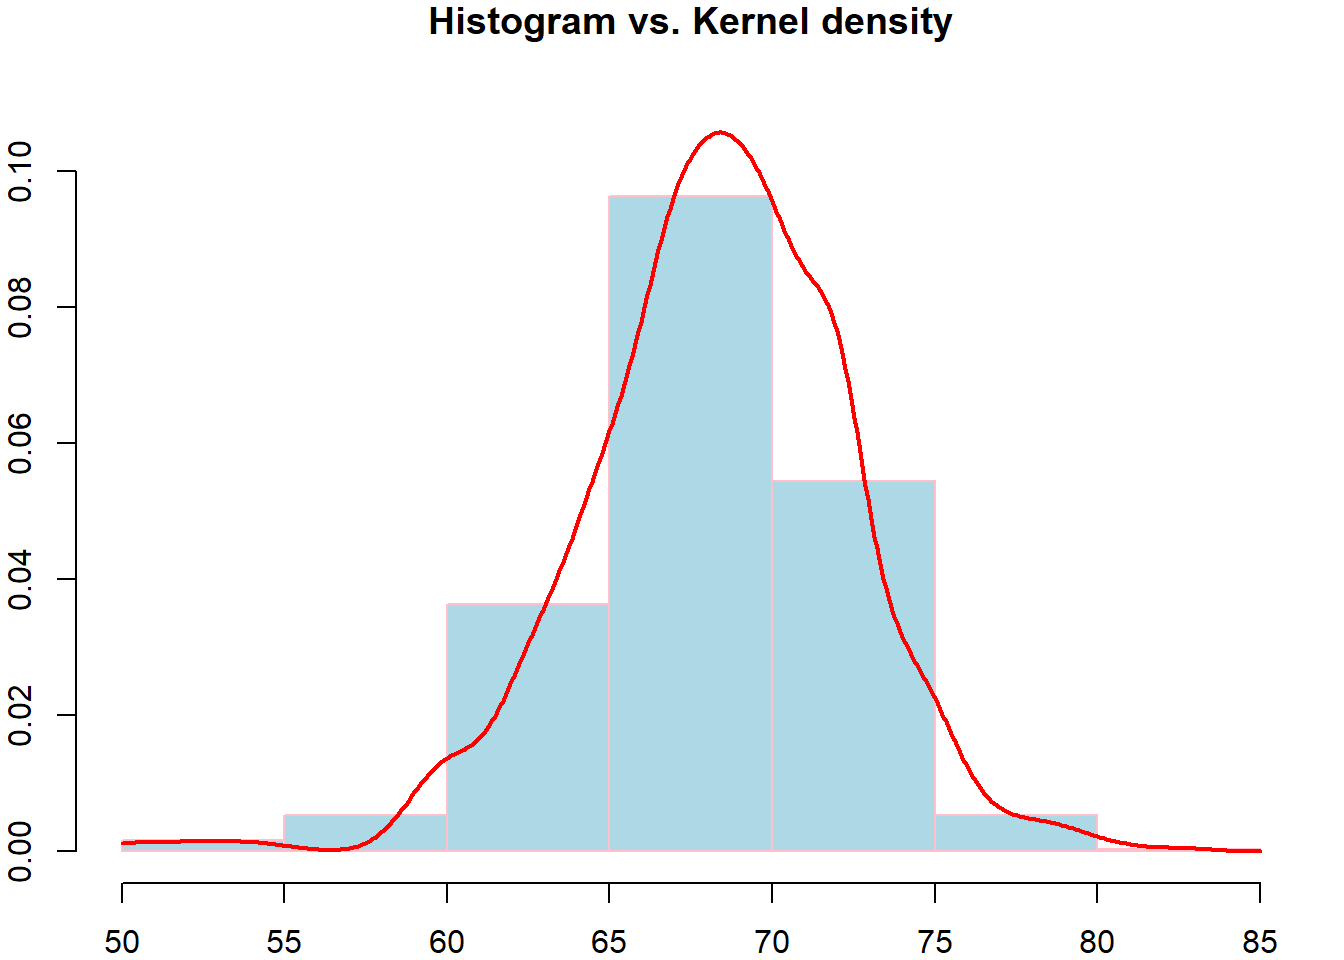
\includegraphics{chap04_files/figure-latex/unnamed-chunk-2-1.pdf}

\begin{Shaded}
\begin{Highlighting}[]
\KeywordTok{summary}\NormalTok{(lm.rod) }\CommentTok{#output the results}
\end{Highlighting}
\end{Shaded}

\begin{verbatim}
## 
## Call:
## lm(formula = finished_weight ~ rough_weight)
## 
## Residuals:
##       Min        1Q    Median        3Q       Max 
## -0.023558 -0.008242  0.001074  0.008179  0.024231 
## 
## Coefficients:
##              Estimate Std. Error t value Pr(>|t|)    
## (Intercept)   0.30773    0.15608   1.972   0.0608 .  
## rough_weight  0.64210    0.05905  10.874 1.54e-10 ***
## ---
## Signif. codes:  0 '***' 0.001 '**' 0.01 '*' 0.05 '.' 0.1 ' ' 1
## 
## Residual standard error: 0.01131 on 23 degrees of freedom
## Multiple R-squared:  0.8372, Adjusted R-squared:  0.8301 
## F-statistic: 118.3 on 1 and 23 DF,  p-value: 1.536e-10
\end{verbatim}

\hypertarget{assessing-the-fit}{%
\subsubsection{Assessing the Fit}\label{assessing-the-fit}}

As an aid in assessing the quality of the fit, we will make extensive
use of the residuals, which are the differences between the observed and
fitted values:
\[\hat e_i = y_i-\hat\beta_0-\hat\beta_1x_i,\ i=1,\dots,n.\]

It is most useful to examine the residuals graphically. Plots of the
residuals versus the \(x\) values may reveal systematic misfit or ways
in which the data do not conform to the fitted model. Ideally, the
residuals should show no relation to the \(x\) values, and the plot
should look like a horizontal blur. The residuals for case study 1 are
plotted below.

\begin{Shaded}
\begin{Highlighting}[]
\KeywordTok{par}\NormalTok{(}\DataTypeTok{mar=}\KeywordTok{c}\NormalTok{(}\DecValTok{4}\NormalTok{,}\DecValTok{4}\NormalTok{,}\DecValTok{2}\NormalTok{,}\DecValTok{1}\NormalTok{))}
\KeywordTok{plot}\NormalTok{(lm.rod}\OperatorTok{$}\NormalTok{fitted.values,lm.rod}\OperatorTok{$}\NormalTok{residuals,}\StringTok{"p"}\NormalTok{,}
     \DataTypeTok{xlab=}\StringTok{"Fitted values"}\NormalTok{,}\DataTypeTok{ylab =} \StringTok{"Residuals"}\NormalTok{)}
\end{Highlighting}
\end{Shaded}

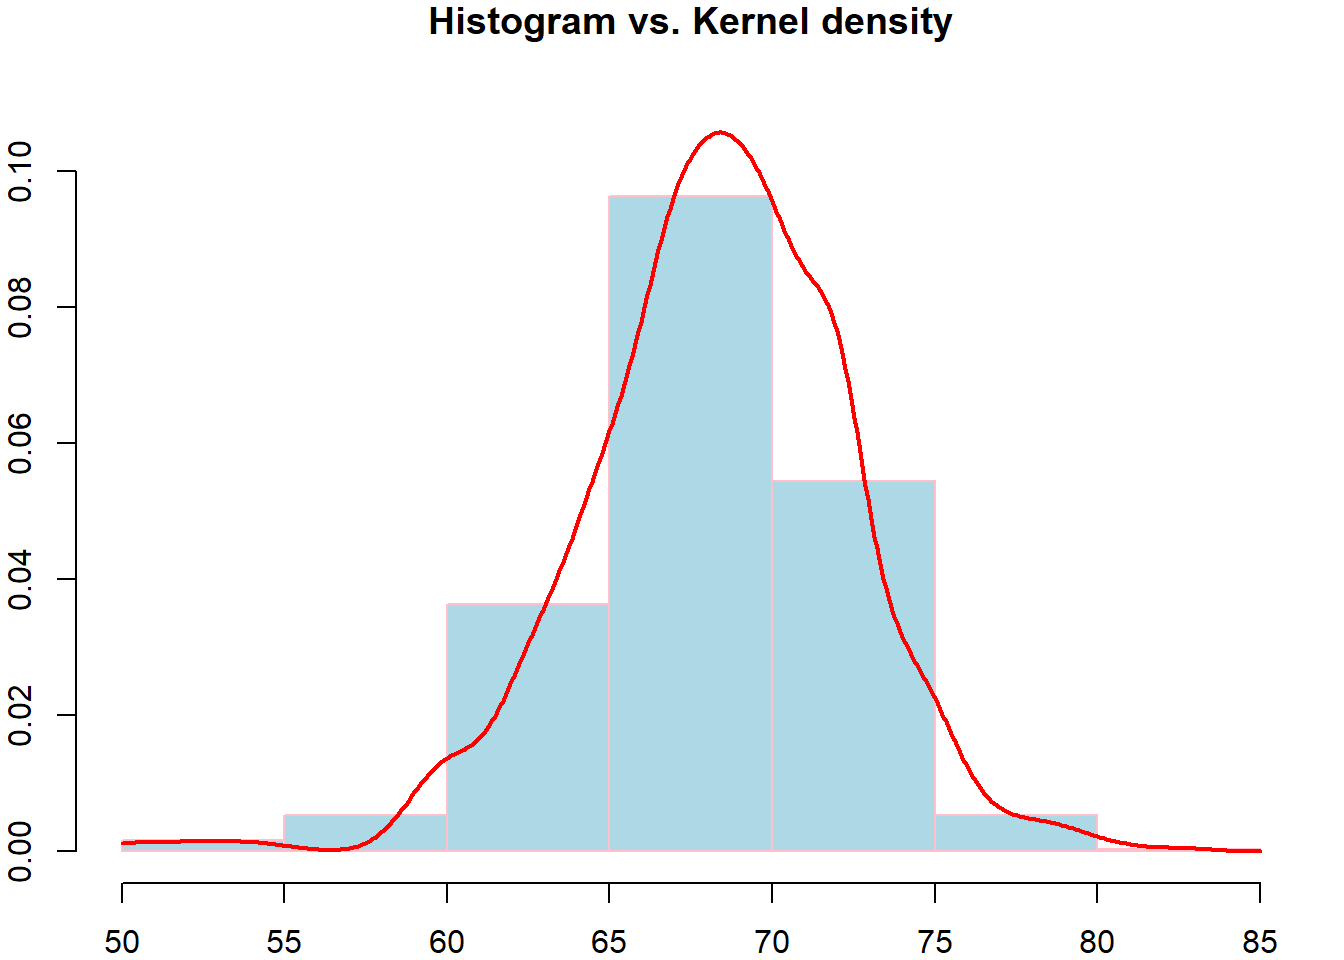
\includegraphics{chap04_files/figure-latex/unnamed-chunk-3-1.pdf}
Standardized Residuals are graphed below. The key command is
\texttt{rstandard}.

\begin{Shaded}
\begin{Highlighting}[]
\KeywordTok{par}\NormalTok{(}\DataTypeTok{mar=}\KeywordTok{c}\NormalTok{(}\DecValTok{4}\NormalTok{,}\DecValTok{4}\NormalTok{,}\DecValTok{2}\NormalTok{,}\DecValTok{1}\NormalTok{))}
\KeywordTok{plot}\NormalTok{(lm.rod}\OperatorTok{$}\NormalTok{fitted.values,}\KeywordTok{rstandard}\NormalTok{(lm.rod),}\StringTok{"p"}\NormalTok{,}
     \DataTypeTok{xlab=}\StringTok{"Fitted values"}\NormalTok{,}\DataTypeTok{ylab =} \StringTok{"Standardized Residuals"}\NormalTok{)}
\KeywordTok{abline}\NormalTok{(}\DataTypeTok{h=}\KeywordTok{c}\NormalTok{(}\OperatorTok{-}\DecValTok{2}\NormalTok{,}\DecValTok{2}\NormalTok{),}\DataTypeTok{lty=}\KeywordTok{c}\NormalTok{(}\DecValTok{5}\NormalTok{,}\DecValTok{5}\NormalTok{))}
\end{Highlighting}
\end{Shaded}

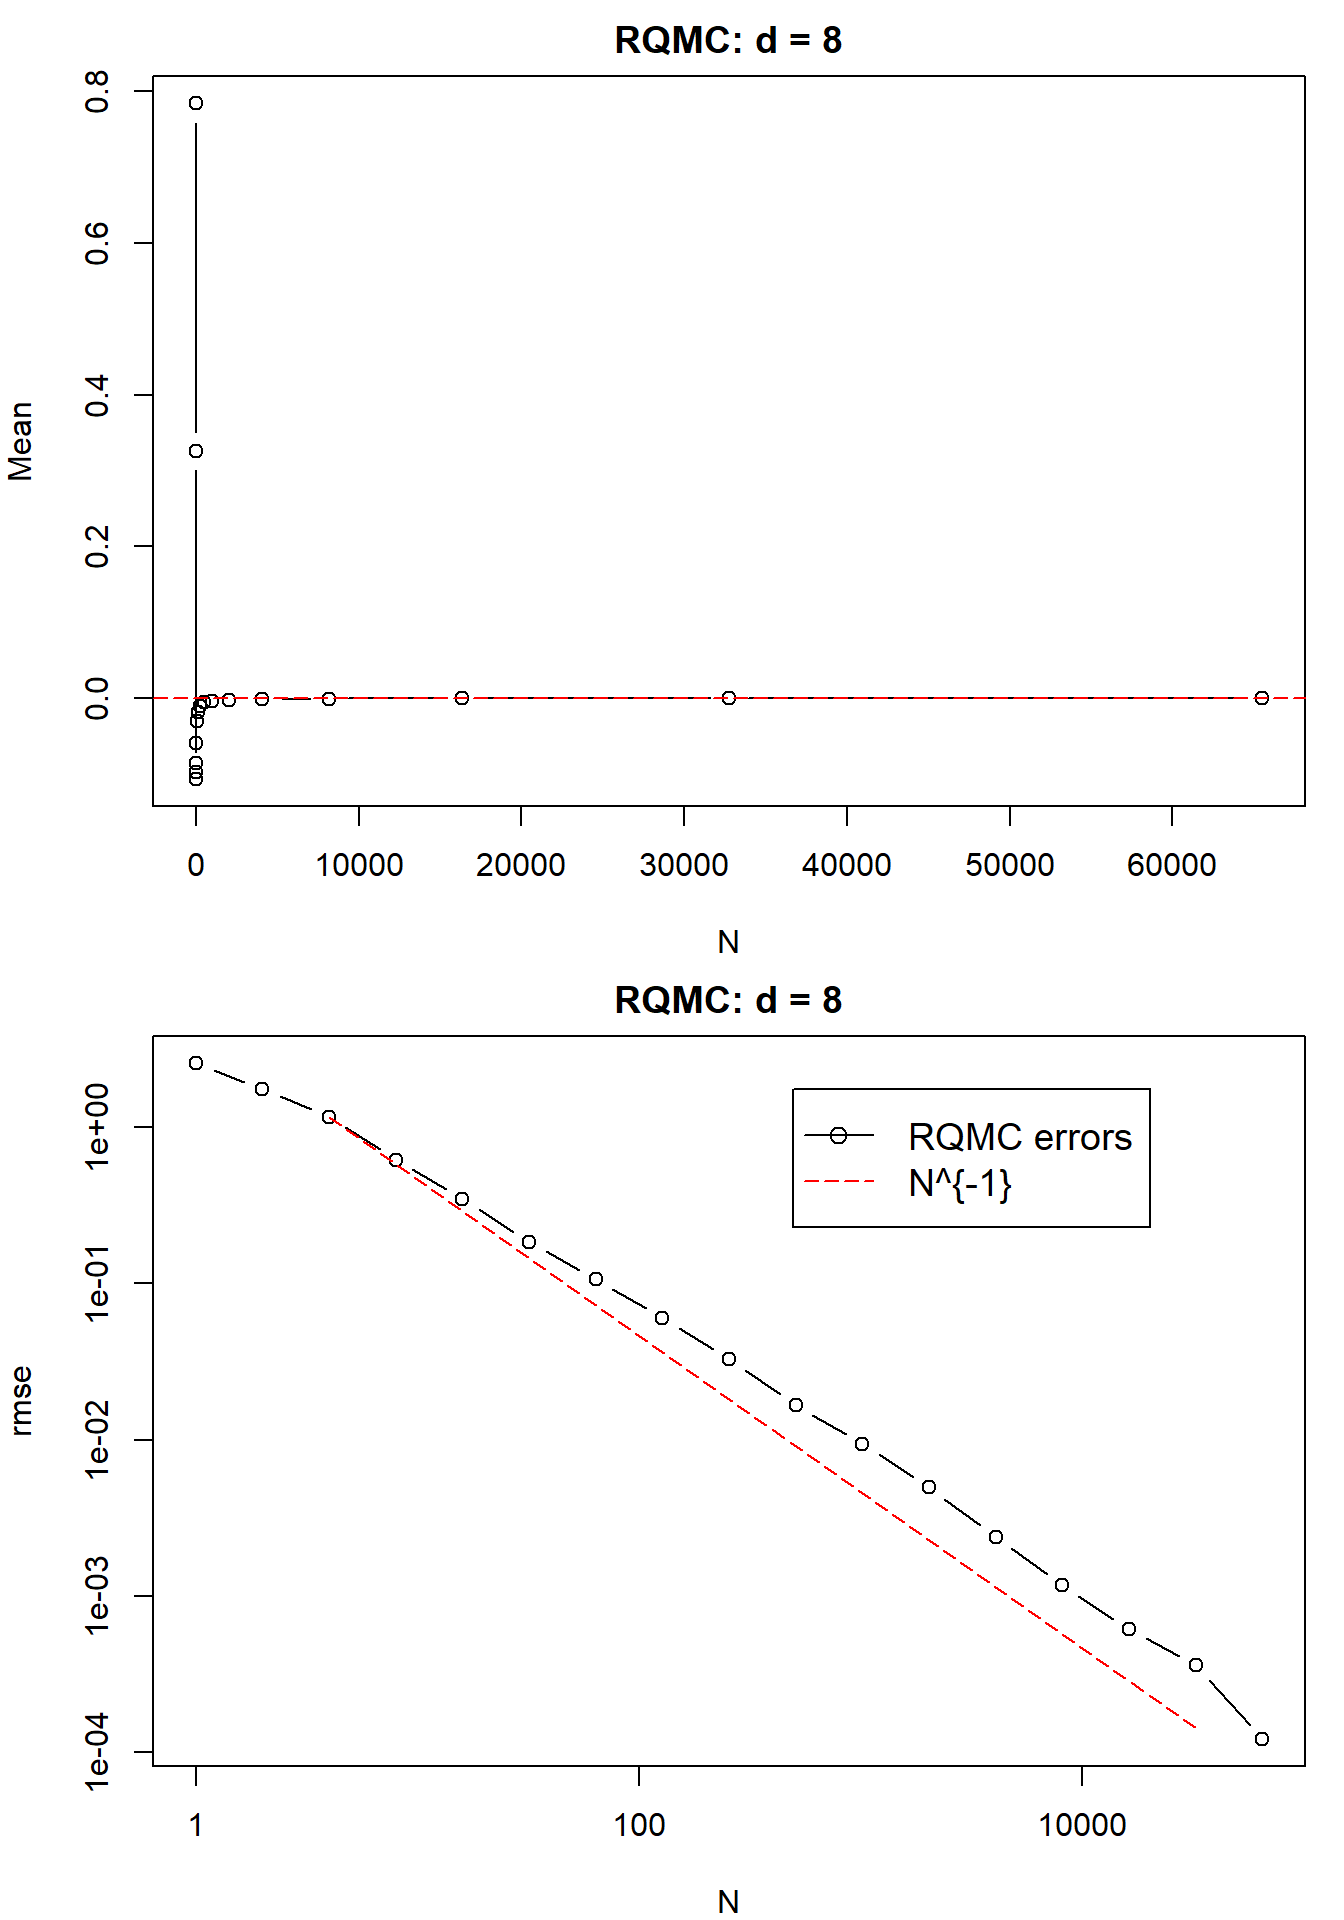
\includegraphics{chap04_files/figure-latex/unnamed-chunk-4-1.pdf}

\hypertarget{drawing-inferences-about-ey}{%
\subsubsection{\texorpdfstring{Drawing Inferences about
\(E[y]\)}{Drawing Inferences about E{[}y{]}}}\label{drawing-inferences-about-ey}}

For given \(x\), we want the estimate the expected value of \(y\), i.e.,
\(E[y]=\beta_0+\beta_1x.\) A natural unbiased estimate is
\(\hat y = \hat\beta_0+\hat\beta_1x\). From the proof of Theorem 3, we
have the variance
\[Var[\hat y] = \left(\frac{1}{n}+\frac{(x-\bar x)^2}{\ell_{xx}}\right)\sigma^2.\]
Under Assumption B, by Theorem 4, we have
\[\hat y\sim N(\beta_0+\beta_1x,(1/n+(x-\bar x)^2/\ell_{xx})\sigma^2),\]
\[\frac{\hat y-E[\hat y]}{\hat{\sigma}\sqrt{1/n+(x-\bar x)/\ell_{xx}}}\sim t(n-2)\]
We thus have the following results.

\texttt{Theorem\ 5}: Suppose Assumption B is satisfied. Then we have
\[\hat y = \hat\beta_0+\hat\beta_1x \sim N(\beta_0+\beta_1x,[1/n+(x-\bar x)^2/\ell_{xx}]\sigma^2).\]
A \(100(1−\alpha)\%\) confidence interval for \(E[y]=\beta_0+\beta_1x\)
is given by
\[\hat y\pm t_{1-\alpha/2}(n-2)\hat{\sigma}\sqrt{\frac{1}{n}+\frac{(x-\bar x)^2}{\ell_{xx}}}.\]

\begin{quote}
Notice from the formula in Theorem 5 that the width of a confidence
interval for \(E[y]\) increases as the value of \(x\) becomes more
extreme. That is, we are better able to predict the location of the
regression line for an \(x\)-value close to \(\bar x\) than we are for
\(x\)-values that are either very small or very large.
\end{quote}

For case study 1, we plot the lower and upper limits for the \(95\%\)
confidence interval for \(E[y]\).

\begin{Shaded}
\begin{Highlighting}[]
\NormalTok{x =}\StringTok{ }\KeywordTok{seq}\NormalTok{(}\FloatTok{2.5}\NormalTok{,}\FloatTok{2.8}\NormalTok{,}\DataTypeTok{by=}\FloatTok{0.001}\NormalTok{)}
\NormalTok{newdata =}\StringTok{ }\KeywordTok{data.frame}\NormalTok{(}\DataTypeTok{rough_weight=}\NormalTok{ x)}
\NormalTok{pred_x =}\StringTok{ }\KeywordTok{predict}\NormalTok{(lm.rod,newdata,}\DataTypeTok{interval =} \StringTok{"confidence"}\NormalTok{)}
\KeywordTok{par}\NormalTok{(}\DataTypeTok{mar=}\KeywordTok{c}\NormalTok{(}\DecValTok{4}\NormalTok{,}\DecValTok{4}\NormalTok{,}\DecValTok{2}\NormalTok{,}\DecValTok{1}\NormalTok{))}
\KeywordTok{matplot}\NormalTok{(x,pred_x,}\DataTypeTok{type=}\StringTok{"l"}\NormalTok{,}\DataTypeTok{lty =} \KeywordTok{c}\NormalTok{(}\DecValTok{1}\NormalTok{,}\DecValTok{5}\NormalTok{,}\DecValTok{5}\NormalTok{),}
        \DataTypeTok{col=}\KeywordTok{c}\NormalTok{(}\StringTok{"blue"}\NormalTok{,}\StringTok{"red"}\NormalTok{,}\StringTok{"red"}\NormalTok{),}\DataTypeTok{lwd=}\DecValTok{2}\NormalTok{,}
        \DataTypeTok{xlab=}\StringTok{"Rough Weight"}\NormalTok{,}\DataTypeTok{ylab=}\StringTok{"Finished Weight"}\NormalTok{)}
\KeywordTok{abline}\NormalTok{(}\DataTypeTok{v=}\KeywordTok{mean}\NormalTok{(rough_weight),}\DataTypeTok{lty=}\DecValTok{5}\NormalTok{)}
\KeywordTok{points}\NormalTok{(rough_weight,finished_weight,}\DataTypeTok{pch=}\DecValTok{16}\NormalTok{)}
\KeywordTok{legend}\NormalTok{(}\FloatTok{2.5}\NormalTok{,}\FloatTok{2.1}\NormalTok{,}\KeywordTok{c}\NormalTok{(}\StringTok{"Fitted"}\NormalTok{,}\StringTok{"Lower limit"}\NormalTok{,}\StringTok{"Upper limit"}\NormalTok{),}
       \DataTypeTok{lty =} \KeywordTok{c}\NormalTok{(}\DecValTok{1}\NormalTok{,}\DecValTok{5}\NormalTok{,}\DecValTok{5}\NormalTok{),}\DataTypeTok{col=}\KeywordTok{c}\NormalTok{(}\StringTok{"blue"}\NormalTok{,}\StringTok{"red"}\NormalTok{,}\StringTok{"red"}\NormalTok{))}
\end{Highlighting}
\end{Shaded}

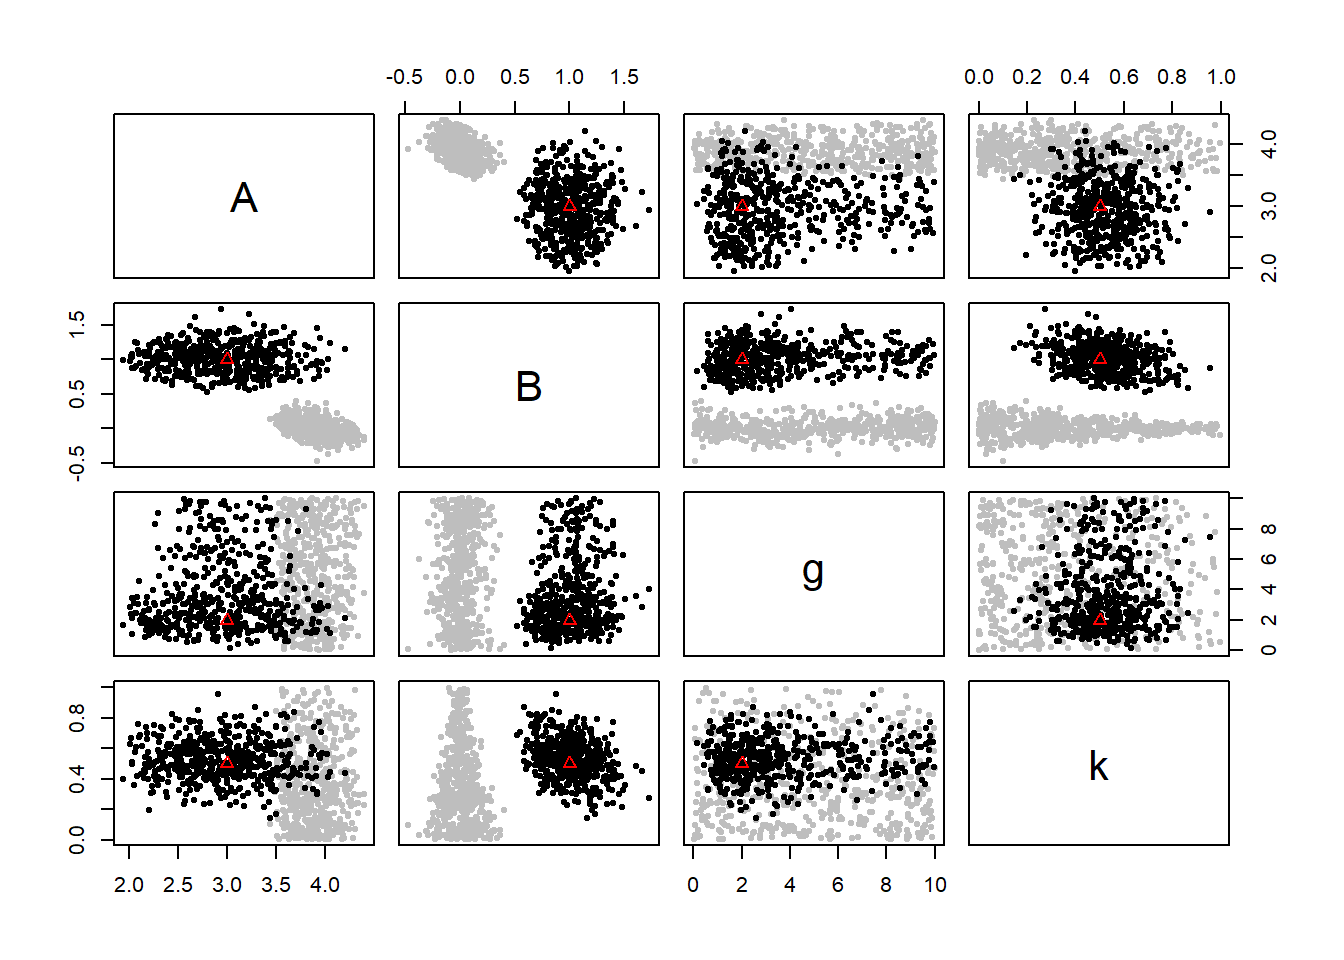
\includegraphics{chap04_files/figure-latex/unnamed-chunk-5-1.pdf}

\hypertarget{drawing-inferences-about-future-observations}{%
\subsubsection{Drawing Inferences about Future
Observations}\label{drawing-inferences-about-future-observations}}

We now give a \textbf{prediction interval} for the future observation
\(y\) rather than its expected value \(E[y]\). Note that here \(y\) is
no longer a fixed parameter, which is assumed to be independent of
\(y_i\)'s. A prediction interval is a range of numbers that contains
\(y\) with a specified probability. Consider \(y-\hat y\). If Assumption
A1 is satisfied, then \[E[y-\hat y] = E[y]-E[\hat y]= 0.\]

If Assumption A2 is satisfied, then
\[Var[y-\hat y] = Var[y]+Var[\hat y]=\left(1+\frac{1}{n}+\frac{(x-\bar x)^2}{\ell_{xx}}\right)\sigma^2.\]

If Assumption B is satisfied, \(y-\hat y\) is then normally distributed.

\texttt{Theorem\ 6}: Suppose Assumption B is satisfied. Let
\(y=\beta_0+\beta_1x+\epsilon\), where \(\epsilon\sim N(0,\sigma^2)\) is
independent of \(\epsilon_i\)'s. A \(100(1−\alpha)\%\) prediction
interval for \(y\) is given by
\[\hat y\pm t_{1-\alpha/2}(n-2)\hat{\sigma}\sqrt{1+\frac{1}{n}+\frac{(x-\bar x)^2}{\ell_{xx}}}.\]

For case study 1, we plot the lower and upper limits for the \(95\%\)
prediction interval for \(y\).

\begin{Shaded}
\begin{Highlighting}[]
\NormalTok{x =}\StringTok{ }\KeywordTok{seq}\NormalTok{(}\FloatTok{2.5}\NormalTok{,}\FloatTok{2.8}\NormalTok{,}\DataTypeTok{by=}\FloatTok{0.001}\NormalTok{)}
\NormalTok{newdata =}\StringTok{ }\KeywordTok{data.frame}\NormalTok{(}\DataTypeTok{rough_weight=}\NormalTok{ x)}
\NormalTok{pred_x =}\StringTok{ }\KeywordTok{predict}\NormalTok{(lm.rod,newdata,}\DataTypeTok{interval =} \StringTok{"prediction"}\NormalTok{)}
\KeywordTok{par}\NormalTok{(}\DataTypeTok{mar=}\KeywordTok{c}\NormalTok{(}\DecValTok{4}\NormalTok{,}\DecValTok{4}\NormalTok{,}\DecValTok{2}\NormalTok{,}\DecValTok{1}\NormalTok{))}
\KeywordTok{matplot}\NormalTok{(x,pred_x,}\DataTypeTok{type=}\StringTok{"l"}\NormalTok{,}\DataTypeTok{lty =} \KeywordTok{c}\NormalTok{(}\DecValTok{1}\NormalTok{,}\DecValTok{5}\NormalTok{,}\DecValTok{5}\NormalTok{),}
        \DataTypeTok{col=}\KeywordTok{c}\NormalTok{(}\StringTok{"blue"}\NormalTok{,}\StringTok{"red"}\NormalTok{,}\StringTok{"red"}\NormalTok{),}\DataTypeTok{lwd=}\DecValTok{2}\NormalTok{,}
        \DataTypeTok{xlab=}\StringTok{"Rough Weight"}\NormalTok{,}\DataTypeTok{ylab=}\StringTok{"Finished Weight"}\NormalTok{)}
\KeywordTok{abline}\NormalTok{(}\DataTypeTok{v=}\KeywordTok{mean}\NormalTok{(rough_weight),}\DataTypeTok{lty=}\DecValTok{5}\NormalTok{)}
\KeywordTok{points}\NormalTok{(rough_weight,finished_weight,}\DataTypeTok{pch=}\DecValTok{16}\NormalTok{)}
\KeywordTok{legend}\NormalTok{(}\FloatTok{2.5}\NormalTok{,}\FloatTok{2.1}\NormalTok{,}\KeywordTok{c}\NormalTok{(}\StringTok{"Fitted"}\NormalTok{,}\StringTok{"Lower limit"}\NormalTok{,}\StringTok{"Upper limit"}\NormalTok{),}
       \DataTypeTok{lty =} \KeywordTok{c}\NormalTok{(}\DecValTok{1}\NormalTok{,}\DecValTok{5}\NormalTok{,}\DecValTok{5}\NormalTok{),}\DataTypeTok{col=}\KeywordTok{c}\NormalTok{(}\StringTok{"blue"}\NormalTok{,}\StringTok{"red"}\NormalTok{,}\StringTok{"red"}\NormalTok{))}
\end{Highlighting}
\end{Shaded}

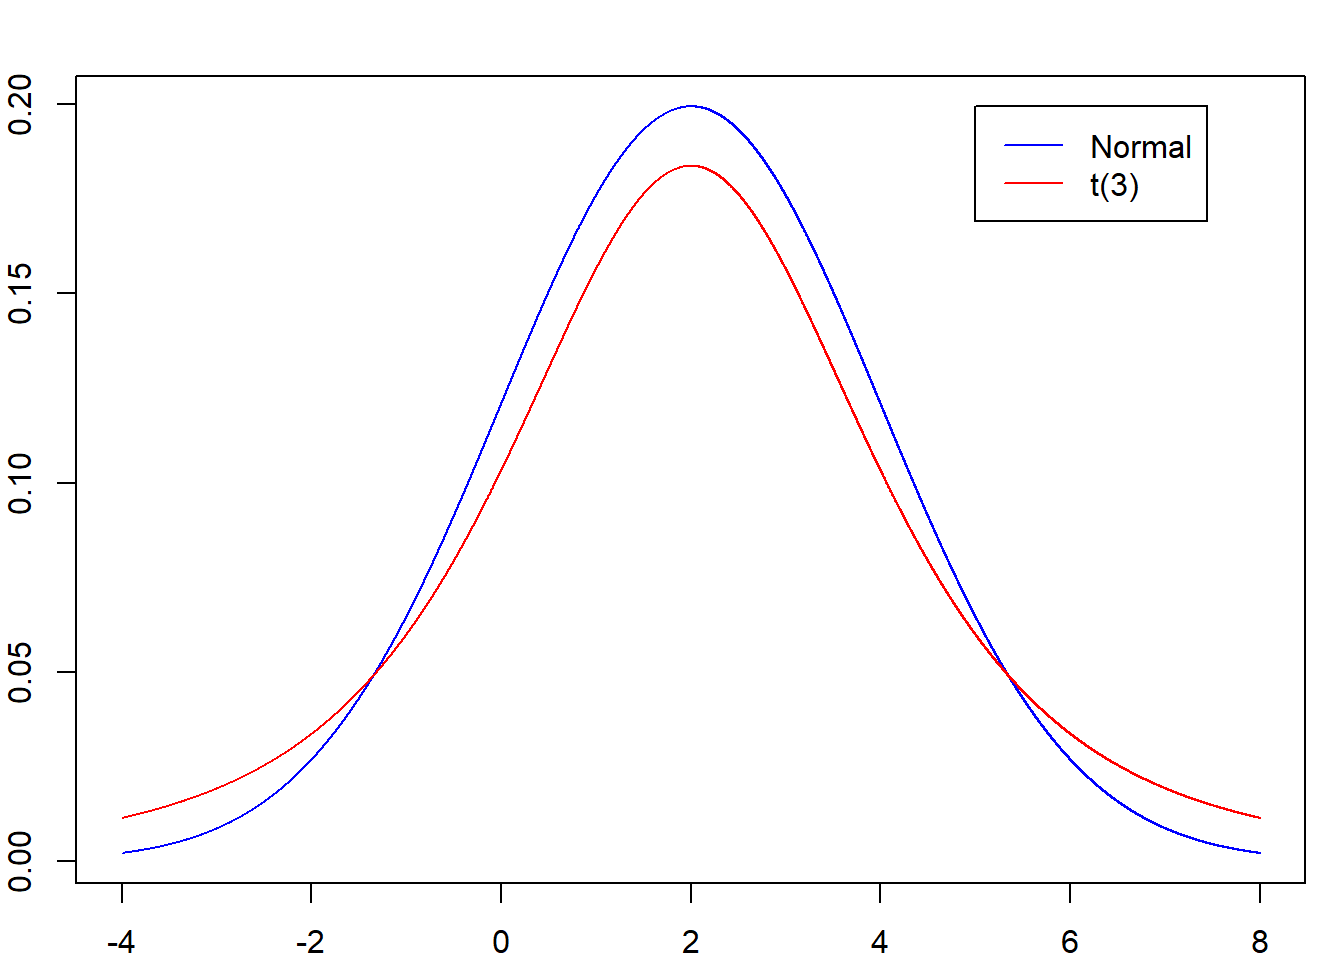
\includegraphics{chap04_files/figure-latex/unnamed-chunk-6-1.pdf}

\hypertarget{how-to-control-y}{%
\subsubsection{How to control y?}\label{how-to-control-y}}

Consider case study 1 again. Castings likely to produce rods that are
too heavy can then be discarded before undergoing the final (and costly)
tooling process. The company's quality-control department wants to
produce the rod \(y\) with weights no large than 2.05. How to choose the
rough casting?

Now we want \(y\le y_0=2.05\) with probability \(1-\alpha\). Similarly
to Theorem 6, we can construct one-side confidence interval for \(y\),
that is
\[\bigg(-\infty,\hat y+t_{1-\alpha}(n-2)\hat{\sigma}\sqrt{1+\frac{1}{n}+\frac{(x-\bar x)^2}{\ell_{xx}}}\bigg].\]
This implies
\[\hat\beta_0+\hat\beta_1x+t_{1-\alpha}(n-2)\hat{\sigma}\sqrt{1+\frac{1}{n}+\frac{(x-\bar x)^2}{\ell_{xx}}}\le y_0.\]

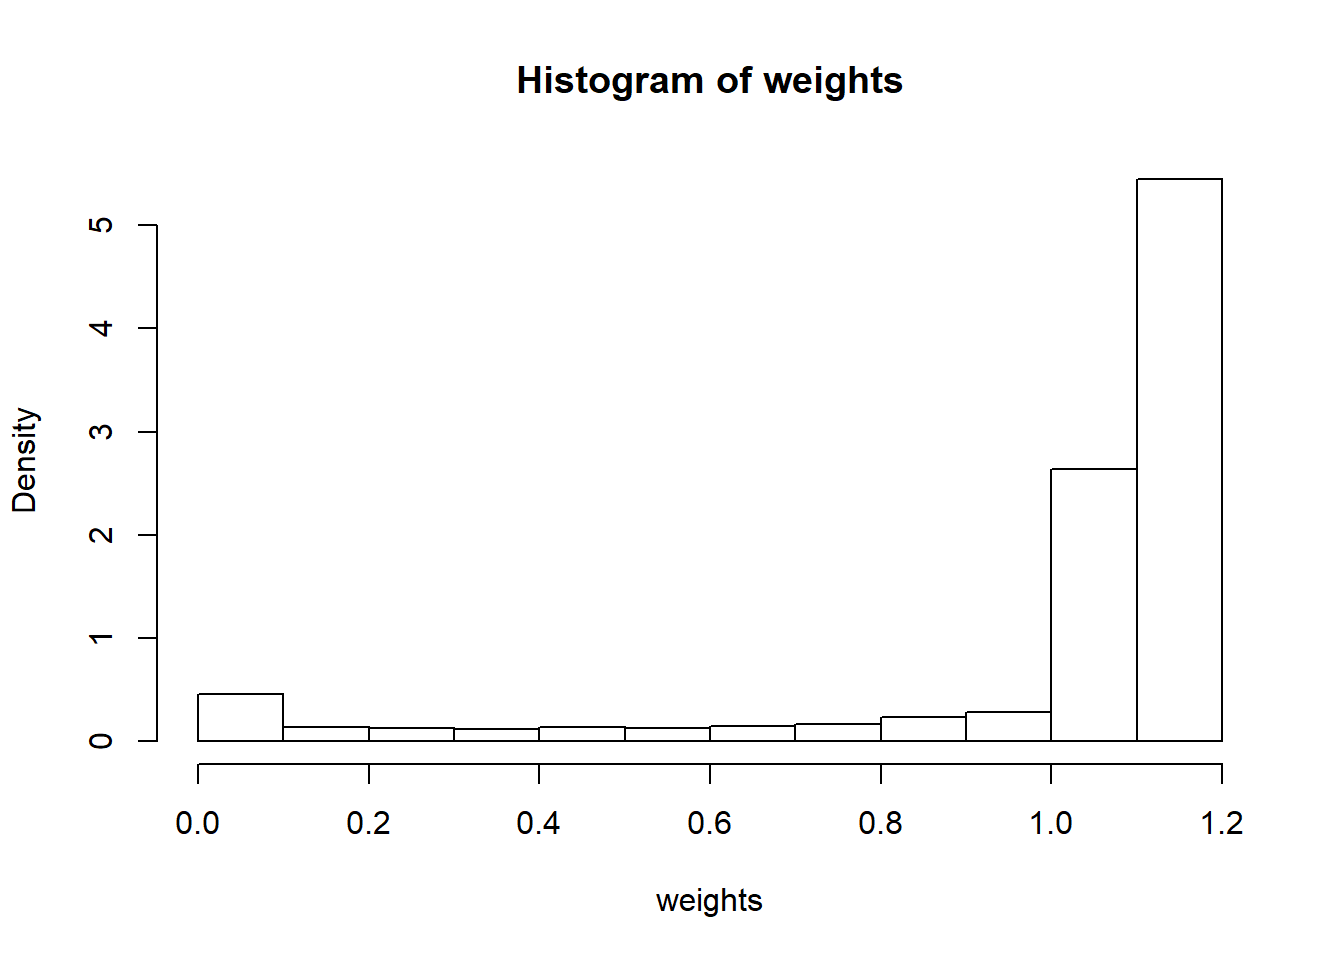
\includegraphics{chap04_files/figure-latex/unnamed-chunk-7-1.pdf}

\hypertarget{multiple-linear-regression}{%
\subsection{Multiple linear
regression}\label{multiple-linear-regression}}

With problems more complex than fitting a straight line, it is very
useful to approach the linear least squares analysis via linear algebra.
Consider a model of the form
\[y_i=\beta_0+\beta_1x_{i1}+\beta_2x_{i2}+\dots+\beta_{p-1}x_{i,p-1}+\epsilon_i,\ i=1,\dots,n.\]

Let \(Y=(y_1,\dots,y_n)^\top\),
\(\beta=(\beta_0,\dots,\beta_{p-1})^\top\),
\(\epsilon=(\epsilon_1,\dots,\epsilon_n)^\top\), and let \(X\) be the
\(n\times p\) matrix \[
X=
\left[
\begin{matrix}
1 & x_{11} & x_{12} & \cdots & x_{1,p-1}\\
1 & x_{21} & x_{22} & \cdots & x_{2,p-1}\\
\vdots & \vdots & \vdots & \vdots & \vdots & \\
1 & x_{n1} & x_{n2} & \cdots & x_{n,p-1}\\
\end{matrix}
\right].
\]

The model can be rewritten as \[Y=X\beta+\epsilon,\]

\begin{itemize}
\item
  the matrix \(X\) is called the \textbf{design matrix},
\item
  assume that \(p<n\).
\end{itemize}

The least squares problem can then be phrased as follows: Find \(\beta\)
to minimize

\[Q(\beta)=\sum_{i=1}^n(y_i-\beta_0-\beta_1x_{i1}-\dots-\beta_{p-1}x_{i,p-1})^2:=||Y-X\beta||^2,\]

where \(||\cdot||\) is the Euclidean norm.

Note that
\[Q=(Y-X\beta)^\top(Y-X\beta) = Y^\top Y-2Y^\top X\beta+\beta^\top X^\top X\beta.\]
If we differentiate \(Q\) with respect to each \(\beta_i\) and set the
derivatives equal to zero, we see that the minimizers
\(\hat\beta_0,\dots,\hat\beta_{p-1}\) satisfy

\[\frac{\partial Q}{\partial \beta_i}=-2(Y^\top X)_i+2(X^{\top}X)_{i\cdot}\hat\beta=0.\]

We thus arrive at \[X^\top X\hat\beta = X^\top Y.\]

If the design matrix \(X^\top X\) is \textbf{nonsingular}, the formal
solution is \[\hat\beta = (X^\top X)^{-1}X^\top Y.\]

The following lemma gives a criterion for the existence and uniqueness
of solutions of the normal equations.

\texttt{Lemma\ 1}: The design matrix \(X^\top X\) is nonsingular if and
only if \(\mathrm{rank}(X)=p\).

\texttt{Proof}: First suppose that \(X^\top X\) is singular. There
exists a nonzero vector \(u\) such that \(X^\top Xu = 0\). Multiplying
the left-hand side of this equation by \(u^\top\), we have
\(0=u^\top X^\top Xu=(Xu)^\top (Xu)\) So \(Xu=0\), the columns of \(X\)
are linearly dependent, and the rank of \(X\) is less than \(p\).

Next, suppose that the rank of \(X\) is less than \(p\) so that there
exists a nonzero vector \(u\) such that \(Xu = 0\). Then
\(X^\top Xu = 0\), and hence \(X^\top X\) is singular.

\begin{quote}
In what follows, we assume that \(\mathrm{rank}(X)=p<n\).
\end{quote}

\hypertarget{expected-values-and-variances}{%
\subsubsection{Expected values and
variances}\label{expected-values-and-variances}}

\texttt{Assumption\ A}: Assume that \(E[\epsilon]=0\) and
\(Var[\epsilon]=\sigma^2I_p\).

\texttt{Theorem\ 7}: Suppose that Assumption A is satisfied and
\(\mathrm{rank}(X)=p<n\), we have

(1). \(E[\hat\beta]=\beta,\)

(2). \(Var[\hat\beta]=\sigma^2(X^\top X)^{-1}\),

\texttt{Proof}:

\[
\begin{align}
E[\hat\beta]&= E[(X^\top X)^{-1}X^{\top}Y] \\
&= (X^\top X)^{-1}X^{\top}E[Y]\\
&=(X^\top X)^{-1}X^{\top}(X\beta)=\beta.
\end{align}\]

\[
\begin{align}
Var[\hat\beta] &= Var[(X^\top X)^{-1}X^{\top}Y]\\
&=(X^\top X)^{-1}X^{\top}Var(Y)X(X^\top X)^{-1}\\
&=\sigma^2(X^\top X)^{-1}.
\end{align}
\]

We used the fact that \(Var(AY) = AVar(Y)A^\top\) for any fixed matrix
\(A\), and \(X^\top X\) and therefore \((X^\top X)^{-1}\) are symmetric.

\hypertarget{estimation-of-sigma2-1}{%
\subsubsection{\texorpdfstring{Estimation of
\(\sigma^2\)}{Estimation of \textbackslash{}sigma\^{}2}}\label{estimation-of-sigma2-1}}

The residual sum of squares (RSS) is defined by
\[\mathrm{RSS}=Q(\hat\beta)=||Y-X\hat\beta||^2=||\hat\epsilon||^2,\]

where the vector of residuals is
\[\hat\epsilon = Y-X(X^\top X)^{-1}X^\top Y:=Y-PY=Y(I_n-P),\]

\begin{itemize}
\tightlist
\item
  \(P=X(X^\top X)^{-1}X^\top\) is an \(n\times n\) matrix (called the
  \textbf{projection matrix}).
\end{itemize}

Two useful properties of \(P\) are given in the following lemma.

\texttt{Lemma\ 2}: Let \(P\) be defined as before. Then
\[P = P^\top=P^2\]

\[I_n-P = (I_n-P)^\top=(I_n-P)^2.\]

\begin{quote}
We may think geometrically of the fitted values, \$\hat Y=X\hat\beta \$,
as being the projection of \(Y\) onto the subspace spanned by the
columns of \(X\).
\end{quote}

The sum of squared residuals is then \[
\begin{align}
\mathrm{SSE} = ||(I_n-P)Y||^2 = Y^\top(I_n-P)^\top(I_n-P)Y=Y^\top(I_n-P)Y.
\end{align}
\]

\texttt{Lemma\ 3}: The cyclic property of the trace, that is,
\(\mathrm{trace}(AB)=\mathrm{trace}(BA)\).

Using Lemma 3, we have

\[
\begin{align}
E[\mathrm{RSS}]&= E[Y^\top(I_n-P)Y]=E[\mathrm{trace}(Y^\top(I_n-P)Y)] \\&= E[\mathrm{trace}((I_n-P)YY^\top)]=\mathrm{trace}((I_n-P)E[YY^\top])\\
&=\mathrm{trace}((I_n-P)(Var[Y]+E[Y]E[Y^\top]))\\
&=\mathrm{trace}((I_n-P)(\sigma^2 I_n))+\mathrm{trace}((I_n-P)X\beta\beta^\top X^\top)\\
&=\sigma^2(n-\mathrm{trace}(P))
\end{align}
\] where we used \((I_n-P)X=X-X(X^\top X)^{-1}X^\top X=0\). Using the
cyclic property of the trace again gives

\[
\begin{align}
\mathrm{trace}(P)&= \mathrm{trace}(X(X^\top X)^{-1}X^\top)\\
&=\mathrm{trace}(X^\top X(X^\top X)^{-1})=\mathrm{trace}(I_p)=p.
\end{align}
\]

We therefore have \(E[\mathrm{RSS}]=(n-p)\sigma^2\).

\texttt{Theorem\ 8}: Suppose that Assumption A is satisfied and
\(\mathrm{rank}(X)=p<n\), \[\hat\sigma^2 = \frac{\mathrm{RSS}}{n-p}\]

is an unbiased estimate of \(\sigma^2\).


\end{document}
